\documentclass[12pt]{article}

\usepackage{fancyhdr} 
\usepackage{amsfonts}
\usepackage{amsmath}
\usepackage{amsthm}
%\usepackage{dsfont}

%\usepackage[scaled]{beramono}
\usepackage{listings}
\usepackage{courier}
\lstset{
	language=Python,
	showstringspaces=false,
	formfeed=newpage,
	tabsize=4,
	commentstyle=\itshape,
	basicstyle=\ttfamily,
}

\usepackage{graphicx}
\graphicspath{ {hw1_images/} }

\usepackage{hyperref}
\hypersetup{
	colorlinks=true,
	linkcolor=blue,
	filecolor=magenta,      
	urlcolor=cyan,
}

\pagestyle{fancy}
\fancyhf{}
\rhead{Shaw \space \thepage}

\setlength\parindent{0pt}

\begin{document}
\thispagestyle{empty}
	
\begin{flushright}
Sage Shaw \\
m565 - Fall 2017 \\
Sep. 9, 2017
\end{flushright}
	
{\large \textbf{HW 1: Problems 1-7}}\bigbreak

	Full Python and C code attached at the end of this document. \bigbreak

%problem 1.a
\hspace{-7 ex}\textbf{1 (a)} Write a program that implements the above algorithm. \bigbreak
	See attached Python code. \\
	Exerpt:
	
	\begin{lstlisting}
		def pi_approx(epsilon):
			pi_approx = []
			
			a = 1
			b = 1/sqrt(2)
			t = 1/4
			j = 1
			while abs(a-b) >= epsilon:
				y = a
				a , b = (a+b)/2 , sqrt(b*y)
				t -= j*(a-y)**2
				j *= 2
				pi_approx.append(a**2/t)
			return pi_approx
	\end{lstlisting}
	
	\bigbreak
	
%problem 1.b
\hspace{-7 ex}\textbf{1 (b) } Run the program with $\epsilon = 10^{-14}$ and report the value of $\tilde{\pi}$ through each iteration of the
while loop in a nice table. Also report the absolute error in between $\tilde{\pi}$ and $\pi$. \bigbreak

	\begin{center}
		\begin{tabular}{|c|c|c|}
			\hline
			$n$ & $\tilde{\pi}$ & $\vert \tilde{\pi} - \pi \vert$ \\ \hline
			1 & 3.1876726427121085 & 0.04607998912231537 \\ \hline
			2 & 3.1416802932976537 & 8.763970786063169e-05 \\ \hline
			3 & 3.1415926538954473 & 3.056541686419223e-10 \\ \hline
			4 & 3.141592653589794 & 8.881784197001252e-16 \\ \hline
		\end{tabular}
	\end{center}
	

	
%problem 1.c
\hspace{-7 ex}\textbf{1 (c) } Make an appropriate plot of the error verses the iteration number. What type of convergence (linear or super-linear) do you observe? \bigbreak

	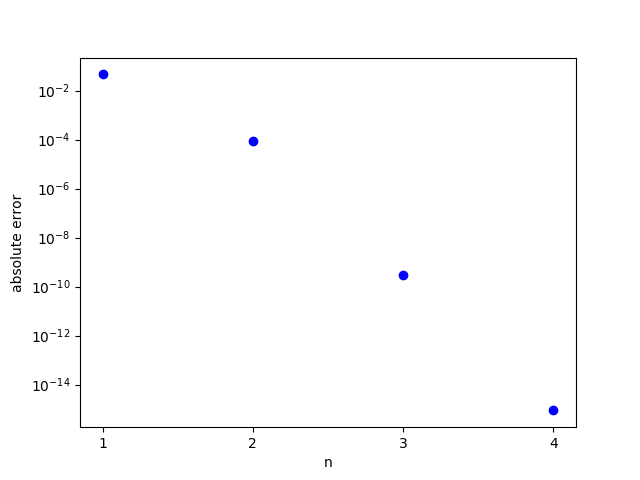
\includegraphics[scale=.65]{Figure_1} \\
	This appears to be super-linear convergence. Note that the error on the 4th and final term is inaccurate due to the precision level. \bigbreak

%problem 1.d
\hspace{-7 ex}\textbf{1 (d) } Show that for any $a_{0} > b_{0} > 0$ that $\{a_{n}\}$ and $\{b_{n}\}$ converge quadratically to
	some number which we will call $M(a_{0}, b_{0})$. \bigbreak
	
	\begin{proof}
		Since $a_{0} > b_{0}$, $a_{1} = \frac{1}{2} (a_{0}+b_{0}) < \frac{1}{2} (a_{0}+a_{0}) = a_{0}$. \\
		Thus $a_{1} < a_{0}$. \\
		Also note $b_{1}^{2} = a_{0}b_{0} > b_{0}^{2}$. Since both sides are positive, $b_{1} > b_{0}$. \\
		Now we show that $b_1<a_1$ as follows:\\
		\begin{align*}
			2a_1 & = a_0 + b_0 \\
			4a_1^2 & = a_0^2 + 2a_0b_0 + b_0^2 \\
			4a_1^2 - 4a_0b_0 & = a_0^2 - 2a_0b_0 + b_0^2 \\
			4(a_1^2 - a_0b_0) & = (a_0 - b_0)^2 > 0\\
			a_1^2 - a_0b_0 & > 0 \\
			a_1^2 - b_1^2 & > 0\\
			a_1 & > b_1\\
		\end{align*}
				
		We now have $0 < b_{0}< b_1 <a_{1} < a_{0}$ which will be our base case. \bigbreak
		
		Now we assume that $0< b_n <a_{n}$ for some $n \in \mathbb{N}$.\\
		Since $b_n < a_n$, $a_{n+1} = \frac{1}{2} (a_{n}+b_{n}) < \frac{1}{2} (a_{n}+a_{n}) = a_{n}$. \\
		Thus $a_{n+1} < a_{n}$. \\
		Also note $b_{n+1}^{2} = a_{n}b_{n} > b_{n}^{2}$. Since both sides are positive, $b_{n+1} > b_{n}$. \\
		Now we show that $b_{n+1}<a_{n+1}$ as follows:\\
		\begin{align*}
		2a_{n+1} & = a_n + b_n \\
		4a_{n+1}^2 & = a_n^2 + 2a_nb_n + b_n^2 \\
		4a_{n+1}^2 - 4a_nb_n & = a_n^2 - 2a_nb_n + b_n^2 \\
		4(a_{n+1}^2 - a_nb_n) & = (a_n - b_n)^2 > 0\\
		a_{n+1}^2 - a_nb_n & > 0 \\
		a_{n+1}^2 - b_{n+1}^2 & > 0\\
		a_{n+1} & > b_{n+1}\\
		\end{align*}
		
		\bigbreak
		
		By induction we have that $b_{n}<b_{n+1}<a_{n+1} < a_{n}$ for all $n \in \mathbb{N}$. \bigbreak
		
		Thus ${a_n}$ is monotonically decreasing and bounded below by $b_0$ and is thus convergent. \\
		Similarly ${b_n}$ is monotonically increasing and bounded above by $a_0$ and is thus convergent. \bigbreak
		
		We now show that $\lim\limits_{n \to \infty}a_n = \lim\limits_{n \to \infty}b_n$. \\
		Note that since $\{a_n\}$ is convergent, it is Cauchy: $\lim\limits_{n \to \infty}\vert a_n - a_{n+1} \vert = 0$. \\
		Also note that $a_{n+1} = \frac{1}{2}(a_n + b_n)$ can be rewritten as $b_n = 2a_{n+1} - a_{n}$. \\
		Then \\
		\begin{align*}
			\lim\limits_{n \to \infty} a_n - \lim\limits_{n \to \infty} b_n  &= \lim\limits_{n \to \infty}\vert a_n - b_n \vert  \\
			& = \lim\limits_{n \to \infty} \vert a_n - 2a_{n+1} + a_{n} \vert  \\
			& = 2\lim\limits_{n \to \infty} \vert a_n - a_{n+1} \vert \\
			& = 0 \\
			\lim\limits_{n \to \infty} a_n & = \lim\limits_{n \to \infty} b_n
		\end{align*}
		
		Define $M(a_{0}, b_{0}) = \lim\limits_{n \to \infty} a_n = \lim\limits_{n \to \infty} b_n$. \bigbreak
		
		We now show that the sequences converge quadratically. by considering the sequence $\{a_n-b_n\} \to 0$. \bigbreak
		
		Let $M = M(a_{0}, b_{0})$. Then \\
		\begin{align*}
			\lim\limits_{n \to \infty} \frac{\vert a_{n+1} - b_{n+1} - 0\vert}{ \vert a_n - b_n - 0 \vert ^ 2} & = \lim\limits_{n \to \infty} \frac{a_{n+1}-b_{n+1}}{(a_n -b_n) ^ 2} \\
			& = \lim\limits_{n \to \infty} \frac{ \frac{1}{2}(a_n+b_n) - \sqrt{a_nb_n}}{(a_n -b_n) ^ 2} \\
			& = \frac{1}{2} \lim\limits_{n \to \infty} \frac{a_n + b_n - 2\sqrt{a_nb_n}}{(a_n -b_n) ^ 2} \\
			& = \frac{1}{2} \lim\limits_{n \to \infty} \frac{(a_n + b_n) - 2\sqrt{a_nb_n}}{(a_n -b_n) ^ 2} * \frac{(a_n + b_n) + 2\sqrt{a_nb_n}}{(a_n + b_n) + 2\sqrt{a_nb_n}}\\
			& = \frac{1}{2} \lim\limits_{n \to \infty} \frac{(a_n + b_n)^2 - 4a_nb_n}{(a_n -b_n) ^ 2 \big( (a_n + b_n) + 2\sqrt{a_nb_n} \big) } \\
			& = \frac{1}{2} \lim\limits_{n \to \infty} \frac{a_n^2 + 2a_nb_n + b_n^2 - 4a_nb_n}{(a_n -b_n) ^ 2 \big( (a_n + b_n) + 2\sqrt{a_nb_n} \big) } \\
			& = \frac{1}{2} \lim\limits_{n \to \infty} \frac{a_n^2 - 2a_nb_n + b_n^2}{(a_n -b_n) ^ 2 \big( (a_n + b_n) + 2\sqrt{a_nb_n} \big) } \\
			& = \frac{1}{2} \lim\limits_{n \to \infty} \frac{(a_n -b_n) ^ 2}{(a_n -b_n) ^ 2 \big( (a_n + b_n) + 2\sqrt{a_nb_n} \big) } \\
			& = \frac{1}{2} \lim\limits_{n \to \infty} \frac{1}{ a_n + b_n + 2\sqrt{a_nb_n} } \\
			& = \frac{1}{2} \frac{1}{ M + M + 2\sqrt{MM} } \\
			& = \frac{1}{8M}
		\end{align*}
		Since $ a_n - M < a_n - b_n$ we can say that $\{a_n\}$ converges quadratically, and since $b_n - M < b_n - a_n$, we can say that $\{b_n\}$ converges quadratically as well, both with convergence constant $\lambda = \frac{1}{8M}$. \\
	\end{proof}
	
	\bigbreak
	
%problem 1.e
\hspace{-7 ex}\textbf{1 (e)} (Extra credit: 5 points) Use high precision arithmetic in your AGM method above to obtain π correctly to at least 100 digits. How many total iterations are needed? Estimate the total number needed to reach at least 1000 digits. \bigbreak

	See attached Python code. \\
	Exerpt: \\
	
	\begin{lstlisting}
	def pi_approx_dec(digits):
		getcontext().prec = digits+2
		epsilon = Decimal(10)**(-1*digits)
		pi_approx = []
		a = Decimal(1)
		b = 1 / Decimal(2).sqrt()
		t = Decimal(1/4)
		j = Decimal(1)
		while abs(a-b) >= epsilon:
			y = a
			a , b = (a+b)/2 , (b*y).sqrt()
			t -= j*(a-y)**2
			j *= 2
			pi_approx.append(a**2/t)
		return pi_approx
	\end{lstlisting}
	
	\bigbreak
	
	\begin{center}
		\begin{tabular}{|c|c|}
			\hline
			$n$ & exponent of absolute error \\ \hline
			1 & -1.33649 \\ \hline
			2 & -4.05730 \\ \hline
			3 & -9.51477 \\ \hline
			4 & -20.42978 \\ \hline
			5 & -42.25980 \\ \hline
			6 & -85.91985 \\ \hline
			7 & -173.23993 \\ \hline
			8 & -347.88011 \\ \hline
			9 & -697.16045 \\ \hline
			10 & -1395.72115 \\ \hline
			11 & -2000.69897 \\ \hline
		\end{tabular}
	\end{center}
	
	From the table, we see that it reaches 100 digits of accuracy by the 7th iteration since it has roughly 172 digits of accuracy. This number needs to double 4 times before it is above 2000, so we would expect to achieve this accuracy on the 11th iteration, which is indeed the case. \bigbreak
	
%probelm 2
\hspace{-7 ex}\textbf{2} Problem 2 uses the Taylor Series for $e^x$ \\
$$ e^x = \lim\limits_{n \to \infty} \sum\limits_{j=0}^{n} \frac{x^j}{j!} $$

\hspace{-7 ex}\textbf{2 (a)} Create a function that computes $e^x$ by truncating the series above to $n$ terms. Using your function for $n = 10$, compute an approximation to $e^x$ for $x = \pm 0.5$ and $x = \pm30\pi$, and report the relative error in your approximation. Repeat these computations for $n = 40$. Comment on your results. \bigbreak

	See attached Python code. \\
	Excerpt: \\
	
	\begin{lstlisting}
def e_taylor(x, n):
	partial_sum = 0
	for i in range(0,n+1):
	partial_sum += x**i / factorial(i)
	return partial_sum
	
def print_hw_output_2a():
	xs = [0.5, -0.5, 30*pi, -30*pi] * 2
	ns = [10]*4 + [40]*4
	for i, (x, n) in enumerate(zip(xs,ns)):
		print('{:.4f}'.format(x), n, 
(exp(x) - e_taylor(x,n)) / exp(x))
	x_labels = ['$0.5$', '$-0.5$', '$30\pi$', '$-30\pi$'] * 2
	rel_errors = [''] * len(x_labels)
	for i, x in enumerate(xs):
		rel_error = abs( (exp(x) - e_taylor(x,ns[i])) / exp(x) )
		rel_errors[i] = "{:.5e}".format(rel_error)
	latex_table( (x_labels, ns, rel_errors), ('$x$', '$n$', 
'relative error'))
	\end{lstlisting}

	\begin{center}
		\begin{tabular}{|c|c|c|}
			\hline
			$x$ & $n$ & relative error \\ \hline
			$0.5$ & 10 & 7.74096e-12 \\ \hline
			$-0.5$ & 10 & -1.93586e-11 \\ \hline
			$30\pi$ & 10 & 1.00000e+00 \\ \hline
			$-30\pi$ & 10 & -1.17500e+54 \\ \hline
			$0.5$ & 40 & 2.69354e-16 \\ \hline
			$-0.5$ & 40 & 1.83045e-16 \\ \hline
			$30\pi$ & 40 & 1.00000e+00 \\ \hline
			$-30\pi$ & 40 & -6.85301e+71 \\ \hline
		\end{tabular}
	\end{center}
	
	For $n=10$, the approximation for small $x$ wasn't bad, but hasn't met the maximum precision for standard double point precision. For $n=40$ the accuracy for small $x$ has reached the machine precision accuracy, roughly. \\
	For large $x$ the relative error is unacceptably large in both cases. \bigbreak
	
\hspace{-7 ex}\textbf{2 (b)} By exploiting properties of the exponential, design an algorithm for accurately computing the value of $e^x$ using the series above, for a wide range of $x$ (e.g. $−100 \leq x \leq 100$). This algorithm can only use the basic operations of the computer described above. Create a function for your algorithm and use it, with $n = 10$, for computing approximations to $e^x$ for $x = \pm0.5$ and $x = \pm 30\pi$. \bigbreak

	Since our approximation above is only good for values of $x$ near $0$, we will use the fact that $$e^x=(e^{\frac{x}{1024}})^{1024}$$ to put our input near zero. See the attached Python code for the implementation. \\
	Excerpt: \\
	\begin{lstlisting}
def e_better_taylor(x,n):
	ret = e_taylor(x/1024,n)
	for i in range(10):
		ret *= ret
	return ret
		
def print_hw_output_2b():
	xs = [0.5, -0.5, 30*pi, -30*pi] * 2
	ns = [10]*4 + [40]*4
	for i, (x, n) in enumerate(zip(xs,ns)):
		print('{:.4f}'.format(x), n, 
(exp(x) - e_taylor(x,n)) / exp(x))	
	x_labels = ['$0.5$', '$-0.5$', '$30\pi$', '$-30\pi$'] * 2
	rel_errors = [''] * len(x_labels)
	for i, x in enumerate(xs):
		rel_error = 
abs( (exp(x) - e_better_taylor(x,ns[i])) / exp(x) )
		rel_errors[i] = "{:.5e}".format(rel_error)
	latex_table( (x_labels, ns, rel_errors), 
('$x$', '$n$', 'relative error'))
	\end{lstlisting}
	
	\begin{center}
		\begin{tabular}{|c|c|c|}
			\hline
			$x$ & $n$ & relative error \\ \hline
			$0.5$ & 10 & 6.41062e-14 \\ \hline
			$-0.5$ & 10 & 4.15512e-14 \\ \hline
			$30\pi$ & 10 & 1.08647e-13 \\ \hline
			$-30\pi$ & 10 & 7.05012e-14 \\ \hline
			$0.5$ & 40 & 6.41062e-14 \\ \hline
			$-0.5$ & 40 & 4.15512e-14 \\ \hline
			$30\pi$ & 40 & 1.08647e-13 \\ \hline
			$-30\pi$ & 40 & 7.05012e-14 \\ \hline
		\end{tabular}
	\end{center}

\hspace{-7 ex}\textbf{2 (c)} Explain how your algorithm from part (b) can be used for approximating cos$(x)$ and sin$(x)$. \bigbreak

	The simplest way to approximate both sin and cos is to use the fact that $e^{i\theta} = \text{cos}(\theta) + i\text{sin}(\theta)$ and use the same algorithm but implemented with complex numbers. By default, Python recognizes complex numbers and uses the appropriate operation based on the type of number object it is passed. This means that we do not even need to reprogram the algorithm, simply pass in complex values. This method is slower however. A faster way, would be to use the Taylor series for either sin or cos and exploit their cyclic and symetric properties to get the inputs in the range of $0 \leq \theta \leq \frac{\pi}{4}$.

%probelm 3
\hspace{-7 ex}\textbf{3 (a)} Verify that the following two functions are identical.\\
	\begin{align*}
		f(x) & = 1 - \text{tan}(x) \\
		g(x) & = \frac{\text{cos}2x}{\text{cos}^2x(1+\text{tan}x)} \\
	\end{align*}
	
	\bigbreak
	
	We will use the facts that $\text{cos}2x = \text{cos}^2x - \text{sin}^2x$ and that $\text{tan}x = \frac{\text{sin}x}{\text{cos}x}$. \\
	\begin{align*}
		g(x) & = \frac{\text{cos}2x}{\text{cos}^2x(1+\text{tan}x)} \\
		& = \frac{\text{cos}^2x - \text{sin}^2x}{\text{cos}^2x(1+\text{tan}x)} \\
		& = \frac{1 - \text{tan}^2x}{1+\text{tan}x} \\
		& = \frac{(1 - \text{tan}x)(1+\text{tan}x)}{1+\text{tan}x} \\
		& = 1 - \text{tan}x \\
		& = f(x)
	\end{align*}
	
\hspace{-7 ex}\textbf{3 (b)} Which function should be used when evaluating $x$ near $\frac{\pi}{4}$ and $\frac{5\pi}{4}$ Why?\bigbreak

	Since tan$x$ is close to $1$ for these values, we should use $g(x)$ to avoid the cancellation error in $f(x)$. \\

\hspace{-7 ex}\textbf{3 (c)} Which function should be used when evaluating $x$ near $\frac{3\pi}{4}$ and $\frac{7\pi}{4}$ Why?\bigbreak

	Since tan$x$ is close to $-1$ for these values, we should use $f(x)$ to avoid the cancellation error in the denominator of $g(x)$. \\

%probelm 4
\hspace{-7 ex}\textbf{4}  Suppose $0 < a < b$. Show that if $\alpha_n = \mathcal{O}(1/n^b)$ as $n \to \infty$ then $\alpha_n = \mathcal{O}(1/n^a)$.\bigbreak

	\begin{proof}
		Since $\alpha_n = \mathcal{O}(1/n^b)$, we can say $\exists C$ such that $\vert \alpha_n \vert \leq C(\frac{1}{n})^b$. \\
		Note that $(\frac{1}{n})^{b} = (\frac{1}{n})^{b-a} (\frac{1}{n})^{a}$. \\
		Then \\
		\begin{align*}
			\vert \alpha_n \vert & \leq C\Big(\frac{1}{n}\Big)^b \\
			\vert \alpha_n \vert & \leq C\Big(\frac{1}{n}\Big)^{b-a} \Big(\frac{1}{n}\Big)^{a} \\
			\vert \alpha_n \vert & \leq \Big(C\frac{1}{n^{b-a}}\Big) \Big(\frac{1}{n}\Big)^{a} \\
		\end{align*}
		For any $n>1$, we can say that $\frac{1}{n^{b-a}} < 1$, and finally $$\vert \alpha_n \vert < C \Big(\frac{1}{n}\Big)^{a}$$. \\
		Thus $\alpha_n = \mathcal{O}(1/n^a)$. \\
	\end{proof}
	
%problem 5
\hspace{-7 ex}\textbf{5}    Suppose we wish to evaluate the integral \\
	\begin{equation*}
			I(N) = \int_{N}^{N+1}\frac{1}{1+x^2}dx
	\end{equation*}
	using the analytical result \\
	\begin{equation}\label{prob2equ3}
		I(N) = \text{arctan}(N+1) - \text{arctan}(N)
	\end{equation}
	
%problem 5a
\hspace{-7 ex}\textbf{5 (a)} Explain why (\ref{prob2equ3}) is unacceptable for computations when $N$ is large, e.g. when $N = 10^8$. \bigbreak

	For large values of $N$, $\text{arctan}(N) \approx 1$, and thus $\text{arctan}(N+1) \approx \text{arctan}(N)$ and we get cancellation error when we compute (\ref{prob2equ3}). \bigbreak
	
%problem 5b
\hspace{-7 ex}\textbf{5 (b)} Find some exact way to re-write (\ref{prob2equ3}) in an acceptable form for computation when $N$ is large. \bigbreak
	
	We will use the trig identity $$ \text{tan}(x-y) = \frac{\text{tan}(x) - \text{tan}(y)}{1 + \text{tan}(x)\text{tan}(y)}$$ to avoid the subtraction as follows: \\
	\begin{align}
		I(N) & = \text{arctan}(N+1) - \text{arctan}(N) \nonumber \\
		\text{tan}\big(I(N)\big) & = \text{tan}\big(\text{arctan}(N+1) - \text{arctan}(N) \big) \nonumber \\
		& = \frac{N + 1 - N}{1 + (N+1)(N)} \nonumber \\
		& = \frac{1}{N^2 + N + 1} \nonumber \\
		I(N) & = \text{arctan}\bigg(\frac{1}{N^2 + N + 1}\bigg) \label{prob5b}
	\end{align}
	
\hspace{-7 ex}\textbf{5 (c)} Compare your formula in Part b with the formula in (\ref{prob2equ3}) for $N = 10^8$. \bigbreak

	Using formula (\ref{prob2equ3}), we compute that $I(N) = 0$. Using formula (\ref{prob5b}), we compute that $I(N) = 9.9999999*10^{-17}$. \bigbreak


%probelm 6
\hspace{-7 ex}\textbf{6 (a)} Implement the cascaded summation function and call it cascsum. \bigbreak

	See attached C code. \\
	Excerpt: \\

	\begin{lstlisting}[language=C]
		double cascsum(double p[], int p_len){
			double e = 0;
			double s = p[0];
			double x, z, y;
			for(int j=1; j<p_len; j++){
				x = p[j] + s;
				z = x - p[j];
				y = (p[j] - (x - z)) + (s - z);
				e += y;
				s = x;
			}
			return s + e;
		}
	\end{lstlisting}	
	
	I attempted to write this in Python, however Python correctly compensated for the error somehow. In \url{https://docs.python.org/3/tutorial/floatingpoint.html} it explains that Python "intelligently" chooses its floating point number representation. I believe that this or something similar is the root of the problem.\\

\hspace{-7 ex}\textbf{6 (b)} Compare the results of your function cascsum to the standard summation algorithm on the following series: \\
	\begin{equation}\label{6bi}
		\sum_{j=1}^{1000000}0.000001
	\end{equation}
	\begin{equation}\label{6bii}
		\sum_{j=0}^{99}(0.99)^j
	\end{equation}
	
	\bigbreak
	
	See below for the program output. \bigbreak
	My C program yielded no error for the cascsum for series (\ref{6bi}), and an error of $\approx 7.918*10^{-12}$ for the regular summation. Clearly the cascsum function is more accurate.\bigbreak
	
	Note that we can calculate the second series without a repeated summation by using this equation $$ \sum_{j=0}^{N}r^j = \frac{1-r^{N+1}}{1-r}$$ We will compare our sums to this value. For the second series we actually have the same number of correct digits for both the sum and the  cascsum, with the error for the sum being slightly less. If summing 200 terms instead of 100, we can see that the accuracy of the cascsum has surpassed the regular sum. And by 400 terms the accuracy of the cascsum is beyond the precision level of this machine. These results give a somewhat mixed message. It seems that there is a point at which the cascsum becomes more accurate than the regular sum.\\
	
	\bigbreak
	
	Program output: \\
	\begin{verbatim}
	For the first series:
	The real sum should be 1.
	Sum     1.0000000000079181
	Cascsum 1.0000000000000000
	Sum error:    -7.9181106116266164e-12
	Cascsum error 0.0000000000000000e+00
	
	For the second series:
	The real sum should be
	        63.39676587267701535211
	Sum     63.39676587267700824668
	Cascsum 63.39676587267702956296
	Sum error:    7.1054273576010019e-15
	Cascsum error -1.4210854715202004e-14
	
	For the second series taken to 200 terms:
	The real sum should be
	86.60203251420374215286
	Sum     86.60203251420369952029
	Cascsum 86.60203251420375636371
	Sum error:    4.2632564145606011e-14
	Cascsum error -1.4210854715202004e-14
	
	For the second series taken to 400 terms:
	The real sum should be
	98.20494467249540093690
	Sum     98.20494467249538672604
	Cascsum 98.20494467249540093690
	Sum error:    1.4210854715202004e-14
	Cascsum error 0.0000000000000000e+00	
	\end{verbatim}


%probelm 7
\hspace{-7 ex}\textbf{7} Consider the sequence defined by $x_{n+1} = x_n(2-ax_n)$ where $0<x_0<2/a$. It can be shown that this sequence converges to $1/a$.\bigbreak

\hspace{-7 ex}\textbf{7 (a)} Illustrate numerically that the sequence converges to $1/5$ with the choice $x_0 = 0.1$. Display the iterates until the relative error between $x_k$ and $1/5$ is $10^{-15}$ or less. \bigbreak

	See attached Python code.
	Excerpt: \\
	
	\begin{lstlisting}
def division(a, x_0=.1, epsilon=10**-15):
	x = x_0
	xs = [x_0]
	n = 0
	ns = [n]
	while abs( (x-(1/a)) *a ) > epsilon:
		n += 1
		x *= (2-a*x)
		ns.append(n)
		xs.append(x)
	return (ns,xs)

def print_hw_output_7():
	(ns, xs) = division(5)
	latex_table((ns,xs), ('$n$', '$x_n$'))
	\end{lstlisting}
	
	Output:\\

	\begin{center}
		\begin{tabular}{|c|c|}
			\hline
			$n$&$x_n$\\ \hline
			0&0.1\\ \hline
			1&0.15000000000000002\\ \hline
			2&0.18750000000000003\\ \hline
			3&0.19921875000000003\\ \hline
			4&0.19999694824218753\\ \hline
			5&0.1999999999534339\\ \hline
			6&0.20000000000000004\\ \hline
		\end{tabular}
	\end{center}
	
\hspace{-7 ex}\textbf{7 (b)} Show mathematically that order of convergence of the sequence to $1/a$ is $2$, and determine $\lambda$. \bigbreak

	We will show this directly \\
	\begin{proof}
		See that \\
		\begin{align*}
			\lim_{n \to \infty} \frac{\vert x_{n+1} - \frac{1}{a} \vert}{\vert x_n - \frac{1}{a} \vert^2} & = \lim_{n \to \infty} \frac{\vert x_n(2-ax_n) - \frac{1}{a} \vert }{\vert x_n^2 - \frac{2}{a}x_n + \frac{1}{a^2} \vert } \\
			& = \lim_{n \to \infty} \frac{\vert -ax_n^2 + 2x_n - \frac{1}{a} \vert }{\vert x_n^2 - \frac{2}{a}x_n + \frac{1}{a^2} \vert } \\
			& = \lim_{n \to \infty} \frac{\vert (-a)(x_n^2 + \frac{2}{a}x_n - \frac{1}{a^2} ) \vert }{\vert x_n^2 - \frac{2}{a}x_n + \frac{1}{a^2} \vert } \\
			& = a \lim_{n \to \infty} \frac{\vert x_n^2 - \frac{2}{a}x_n + \frac{1}{a^2} \vert }{\vert x_n^2 - \frac{2}{a}x_n + \frac{1}{a^2} \vert } \\
			& = a \\
		\end{align*}
		Thus $\{x_n\}$ converges quadratically with $\lambda = a$. \\
	\end{proof}

\end{document}
